\section{Variedades proyectivas}

\begin{preliminaries}
Sean $V \subset \P^n$ una variedad proyectiva, tal y como definimos a continuación. Sea $C \subset \A^{n+1}$ el cono afín sobre $V$.
\end{preliminaries}

\begin{definition}
Una \textit{variedad proyectiva} es un conjunto algebraico proyectivo vacío o irreducible.
\end{definition}

\begin{definition}
Una \textit{función homogénea} sobre $C$ es una función regular $f : C \to k$ que puede ser expresada como la restricción a $C$ de una función homogénea $\bar f : \A^{n+1} \to k$.
\end{definition}

\begin{definition}
El \textit{anillo de coordenadas homogéneo} de $V$ es $k_h[V] = k[C]$.
\end{definition}

\begin{remark}
Dos funciones homogéneas $f, g : \A^{n+1} \to k$ inducen la misma función homogénea sobre $V$ si y sólo si $f - g \in I(V)$. Por ende, $k_h[V]$ es naturalmente isomorfo a $k_h[\P^n] / I(V)$.
\end{remark}

\begin{proposition}
Sea $f : C \to k$ una función regular. Existe una única sucesión de funciones homogéneas $f_r : C \to k$ tales que $f = \sum_r f_r$ y $\deg f_r = r$. Además, sólo un número finito de ellas son distintas de cero.
\end{proposition}

\begin{proof}
Ver \cite[p. 92]{fulton}.
\end{proof}

\begin{definition}
El \textit{cuerpo de funciones racionales} sobre $V$, denotado $k(V)$, está conformado por los cocientes $f/g$, donde $f, g : C \to k$ son funciones homogéneas del mismo grado y $g$ no es la función idénticamente nula.
\end{definition}

\begin{remark}
Las reglas usuales para manipular fracciones son válidas en $k(V)$. En particular, si $f, g$ tienen un factor común, podemos simplificar dicho factor sin alterar el cociente.
\end{remark}

\begin{figure}[h]
    \centering
    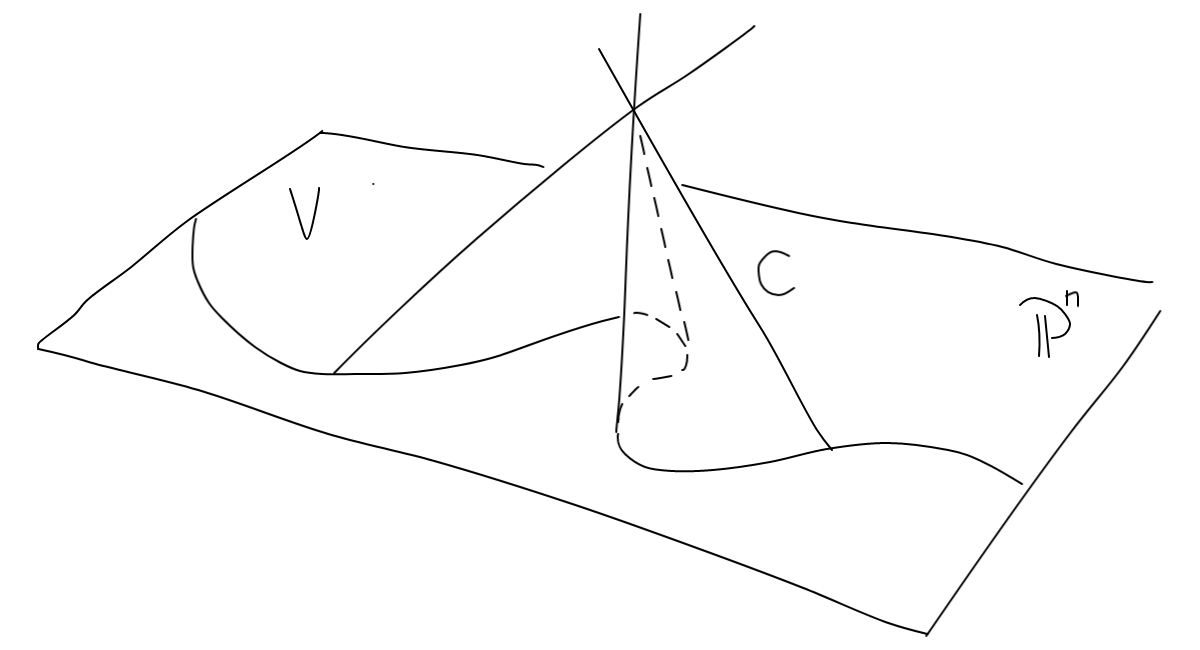
\includegraphics[scale=0.3]{ch2/cone.png}
    \caption[Cono sobre una variedad proyectiva]{Cono sobre una variedad proyectiva \cite[p. 12]{hartshorne}}
\end{figure}

\begin{definition}
Sea $z \in k(V)$ una función racional. Decimos que $z$ está \textit{definida} en $p \in V$ si existen funciones homogéneas $f, g : C \to k$ tales que $z = f/g$ y además $g(p) \ne 0$. Decimos que $z$ se \textit{anula} en $p$ si, además, $f(p) = 0$.
\end{definition}

\begin{definition}
El \textit{anillo local} de $V$ en el punto $p \in V$, denotado $\O_p(V)$, está conformado por todas las funciones racionales $z \in k(V)$ definidas en $p$.
\end{definition}

\begin{remark}
Si $z \in k(V)$ no se anula en $p$, entonces $z^{-1}$ está definida en $p$, por ende...
\end{remark}

\begin{definition}
El único \textit{ideal maximal} de $\O_p(V)$, denotado $\m_p(V)$, está conformado por todas las funciones racionales $z \in k(V)$ que se anulan en $p$.
\end{definition}

\begin{remark}
En general, diremos que un anillo es \textit{local} si tiene un único ideal maximal.
\end{remark}

\begin{definition}
Una \textit{función regular} sobre un subconjunto abierto de Zariski $U \subset V$ es una función racional sobre $V$ que está definida en todo punto $p \in U$.
\end{definition}

\begin{corollary}
Toda función regular sobre una variedad proyectiva es constante.
\end{corollary}
